\documentclass{article}
% \usepackage{fullpage}

\usepackage{template}

\usepackage{tikz}
\usetikzlibrary{positioning,fit,calc}

\header{%
  assignment={\texttt{mininet} Guide},%
  course={IN[59]570: Distributed Objects},%
  authors={Oleks Shturmov \texttt{<\href{mailto:oleks@oleks.info}{oleks@oleks.info}>}},%
  affiliation={Department of Informatics\\University of Oslo},%
  shortAffiliation={IFI/UiO},%
  date={\today}%
}

\newcommand{\mininet}{\texttt{mininet}}

\begin{document}

\maketitle

\mininet{} is a tool for light-weight computer network emulation. To
this end it uses operating-system (OS) level virtualisation, similar
to ``container'' technologies like Docker. \mininet{} allows us to
test that our distributed software behaves as expected in various
concrete computer networking scenarios.

You can either install \mininet{} natively; or run it in a VM, or a
container. We recommend one of the latter options since \mininet{},
rather unfortunately, \underline{\textbf{requires root priveleges for
network emulation}}. That said, there is no need to expose your
personal machine, or network, to \mininet{}. Using a container or a VM
allows you to hand \mininet{} its desired privileges, but only to a
confined, simulated machine. Figure \ref{fig:mininet-basics}
illustrates the setup we will create.

\begin{figure}[h!]
\centering

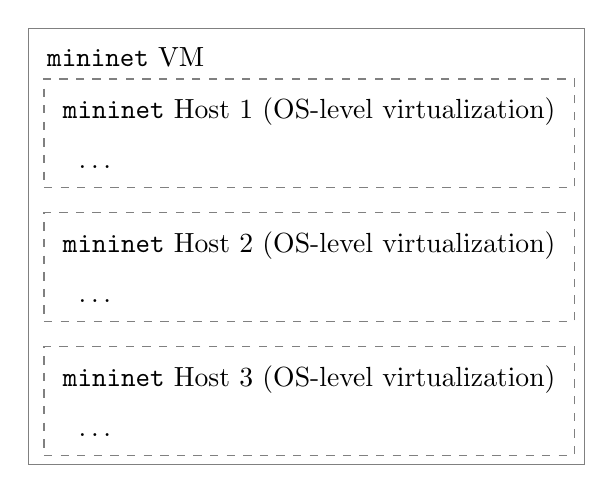
\begin{tikzpicture}[
  node distance=7mm,
  title/.style={},
  subtitle/.style={anchor=west},
  typetag/.style={anchor=west}
]
  \node (vm) [title] { \texttt{mininet} VM };

  \node (h1) [below=of vm.west, subtitle, xshift=2mm] { \texttt{mininet} Host 1 (OS-level virtualization) };
  \node (d1) [below=of h1.west, typetag, xshift=2mm] { \ldots };

  \node (h1wrap) [draw=black!50, fit={(h1) (d1)}, dashed] {};

  \node (h2) [below=of h1.west, subtitle, yshift=-10mm] { \texttt{mininet} Host 2 (OS-level virtualization) };
  \node (d2) [below=of h2.west, typetag, xshift=2mm] { \ldots };

  \node (h2wrap) [draw=black!50, fit={(h2) (d2)}, dashed] {};

  \node (h3) [below=of h2.west, subtitle, yshift=-10mm] { \texttt{mininet} Host 3 (OS-level virtualization) };
  \node (d3) [below=of h3.west, typetag, xshift=2mm] { \ldots };

  \node (h3wrap) [draw=black!50, fit={(h3) (d3)}, dashed] {};

  \node [draw=black!50, fit={(vm) (h1wrap) (h2wrap) (h3wrap)}] {};

\end{tikzpicture}


\caption{Illustration of a \mininet{} setup; with \mininet{} running
in the official \mininet{} VM, emulating 3 hosts. We use a solid line
to indicate a solid virtualization boundary, and dashed lines for a
softer, OS-level one. }

\label{fig:mininet-basics}

\end{figure}

Not only does running \mininet{} in a dedicated VM provide for a solid
boundary between our experiments and your personal machine, it is also
the recommended way to get started according to the official
documentation:

\begin{center}

\url{https://mininet.org/download/\#option-1-mininet-vm-installation-easy-recommended}

\end{center}

After you download and setup the VM with your favourite virtualisation
technology (e.g., VirtualBox, VMware Fusion, QEMU); we can recommend
to setup SSH port-forwarding, and connect to the VM via SSH. This is
done by configuring the VM in your virtualisation software.

\textbf{We will assume that you set host port 8022 to be forwarded to
port 22 (SSH port) inside the VM}. However, if your port 8022 is taken
by some other software, feel free to use another port.

\textbf{The username is \texttt{mininet}, so is the password}, and
password-based login via SSH is enabled by default. Here, we have no need
to harden this boundary.

If everything is setup correctly, you should be able to do the
following in your favourite command-line shell:

\begin{lstlisting}
$ ssh -p 8022 mininet@localhost
mininet@localhost's password: mininet
Welcome to Ubuntu 20.04.6 LTS (GNU/Linux 5.4.0-205-generic x86_64)

 * Documentation:  https://help.ubuntu.com
 * Management:     https://landscape.canonical.com
 * Support:        https://ubuntu.com/pro
New release '22.04.5 LTS' available.
Run 'do-release-upgrade' to upgrade to it.

Last login: Wed Feb 19 02:30:13 2025 from 10.0.2.2
mininet@mininet-vm:~$
\end{lstlisting}



\end{document}
